%%%%%%%%%%%%%%%%%%%%%%%%%%%%%%%%%%%%%%%%%%%%%%%%%%%%%%%%%%%%%%%%%%%%%%%%%%%%%%%
% Chapter 'Absorption - Water - LiBr/H2N(CH2)2OH  ratio 3/5/1'
%%%%%%%%%%%%%%%%%%%%%%%%%%%%%%%%%%%%%%%%%%%%%%%%%%%%%%%%%%%%%%%%%%%%%%%%%%%%%%%
\subsection{Libr/h2n(ch2)2oh  ratio 3/5/1}
%
%%%%%%%%%%%%%%%%%%%%%%%%%%%%%%%%%%%%%%%%%%%%%%%%%%%%%%%%%%%%%%%%%%%%%%%%%%%%%%%
%%%%%%%%%%%%%%%%%%%%%%%%%%%%%%%%%%%%%%%%%%%%%%%%%%%%%%%%%%%%%%%%%%%%%%%%%%%%%%%
\subsubsection{Antoine - ID 1}
%
\begin{tabular}[l]{|lp{11.5cm}|}
\hline
\addlinespace

\textbf{Sorbent:} & LiBr/H2N(CH2)2OH  \\
\textbf{Subtype:} & ratio 3/5/1 \\
\textbf{Refrigerant:} & Water \\
\textbf{Equation:} & Antoine \\
\textbf{ID:} & 1 \\
\textbf{Reference:} & Kim, Jin-Soo; Park, Young; Lee, Huen (1996): Densities and Viscosities of the Water + Lithium Bromide + Ethanolamine System. In: J. Chem. Eng. Data 41 (4), S. 678–680. DOI: 10.1021/je9503259. \\
\textbf{Comment:} & None \\

\addlinespace
\hline
\end{tabular}
\newline

\textbf{Equation and parameters:}
\newline
%
Pressure $p$ in $\si{\pascal}$ is calculated depending on concentration $X$ in $\si{\kilogram\per\kilogram}$ and  temperature $T$ in $\si{\kelvin}$ by:
%
\begin{equation*}
\nicefrac{p}{d} = 10 ^ { \sum_{i=0}^{4} \left( A_i + \frac{1000 B_i}{T - c} \right) \left( 100 X \right) ^{i}}
\end{equation*}
%
The parameters of the equation are:
%
\begin{longtable}[l]{lll|lll}
\toprule
\addlinespace
\textbf{Par.} & \textbf{Unit} & \textbf{Value} &	\textbf{Par.} & \textbf{Unit} & \textbf{Value} \\
\addlinespace
\midrule
\endhead

\bottomrule
\endfoot
\bottomrule
\endlastfoot
\addlinespace

$c$ & $\si{\kelvin}$ & 4.315000000e+01 & $d$ & $\si{\pascal}$ & 1.000000000e+03 \\
$A_0$ & - & 1.227900000e+02 & $B_0$ & $\si{\kelvin}$ & -3.833350000e+01 \\
$A_1$ & - & -7.188120000e+00 & $B_1$ & $\si{\kelvin}$ & 2.259820000e+00 \\
$A_2$ & - & 1.658530000e-01 & $B_2$ & $\si{\kelvin}$ & -5.165830000e-02 \\
$A_3$ & - & -1.688300000e-03 & $B_3$ & $\si{\kelvin}$ & 5.197140000e-04 \\
$A_4$ & - & 6.412610000e-06 & $B_4$ & $\si{\kelvin}$ & -1.956930000e-06 \\

\addlinespace\end{longtable}

\textbf{Validity:}
\newline
Equation is approximately valid for $318.15 \si{\kelvin} \leq T \leq 418.15 \si{\kelvin}$.
\newline

\textbf{Visualization:}
%
\begin{figure}[!htp]
{\noindent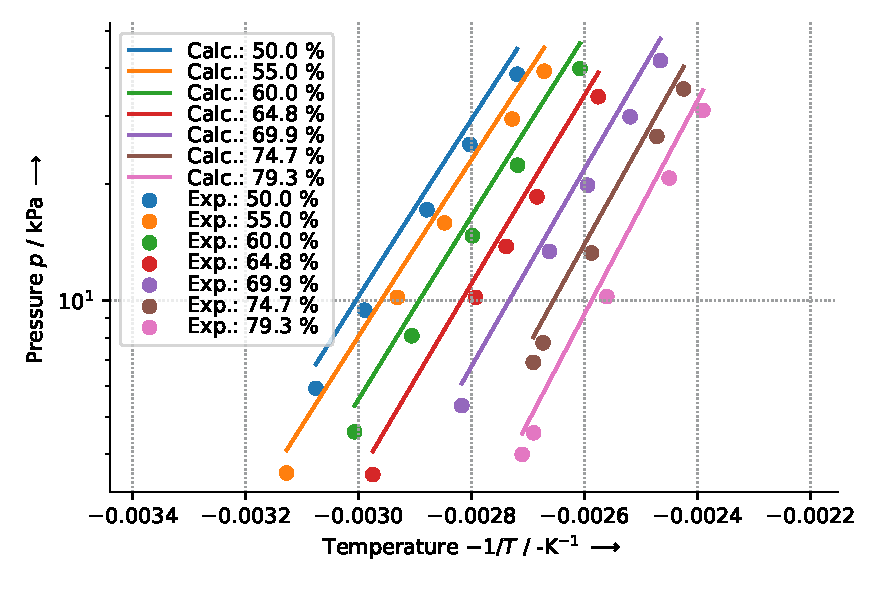
\includegraphics[height=10cm, keepaspectratio]{figs/abs/abs_Water_LiBr_H2N(CH2)2OH__ratio_3_5_1_Antoine_1.pdf}}
\end{figure}
%

To generate the figure, the following refrigerant functions were selected:
\begin{itemize}
\item Vapor pressure: VaporPressure\_EoS1 - ID 1
\item Saturated liquid density: SaturatedLiquidDensity\_EoS1 - ID 1
\end{itemize}

The uncertainity of the experimental data is:
\begin{itemize}
\item Data source $\,\to\,$ Data was taken from table
\item Temperature, relative, in \% $\,\to\,$ 0.4
\end{itemize}

The mean absolute percentage error (MAPE) between the experimental and calculated data results in 14.58\%.
\FloatBarrier
\newpage
%%%%%%%%%%%%%%%%%%%%%%%%%%%%%%%%%%%%%%%%%%%%%%%%%%%%%%%%%%%%%%%%%%%%%%%%%%%%%%%
